\chapter{Software Components or Modules needed} 
% Main chapter title

\label{Chapter6} 
%Call reference to this chapter use \ref{ChapterX}

\lhead{Chapter 6. \emph{Software Components or Modules needed}} 
% Change X to a consecutive number; this is for the header on each page - perhaps a shortened title

\doublespacing
% LINE FORMATTING

%\clearpage
%\pagebreak
\section{Software Components and Modules needed}
Below the list that shows and, descripe components and modules needed to build MTS.

\begin{description}
	\item[Web server] description
	\item[Backup server] description
	\item[Database] description
	
\end{description}

% MAIN SECTION ==============================
\pagebreak
\section{Software Architecture}
Below is an architecture diagram shows the software architecture.
\begin{figure}[H]
	\centering
	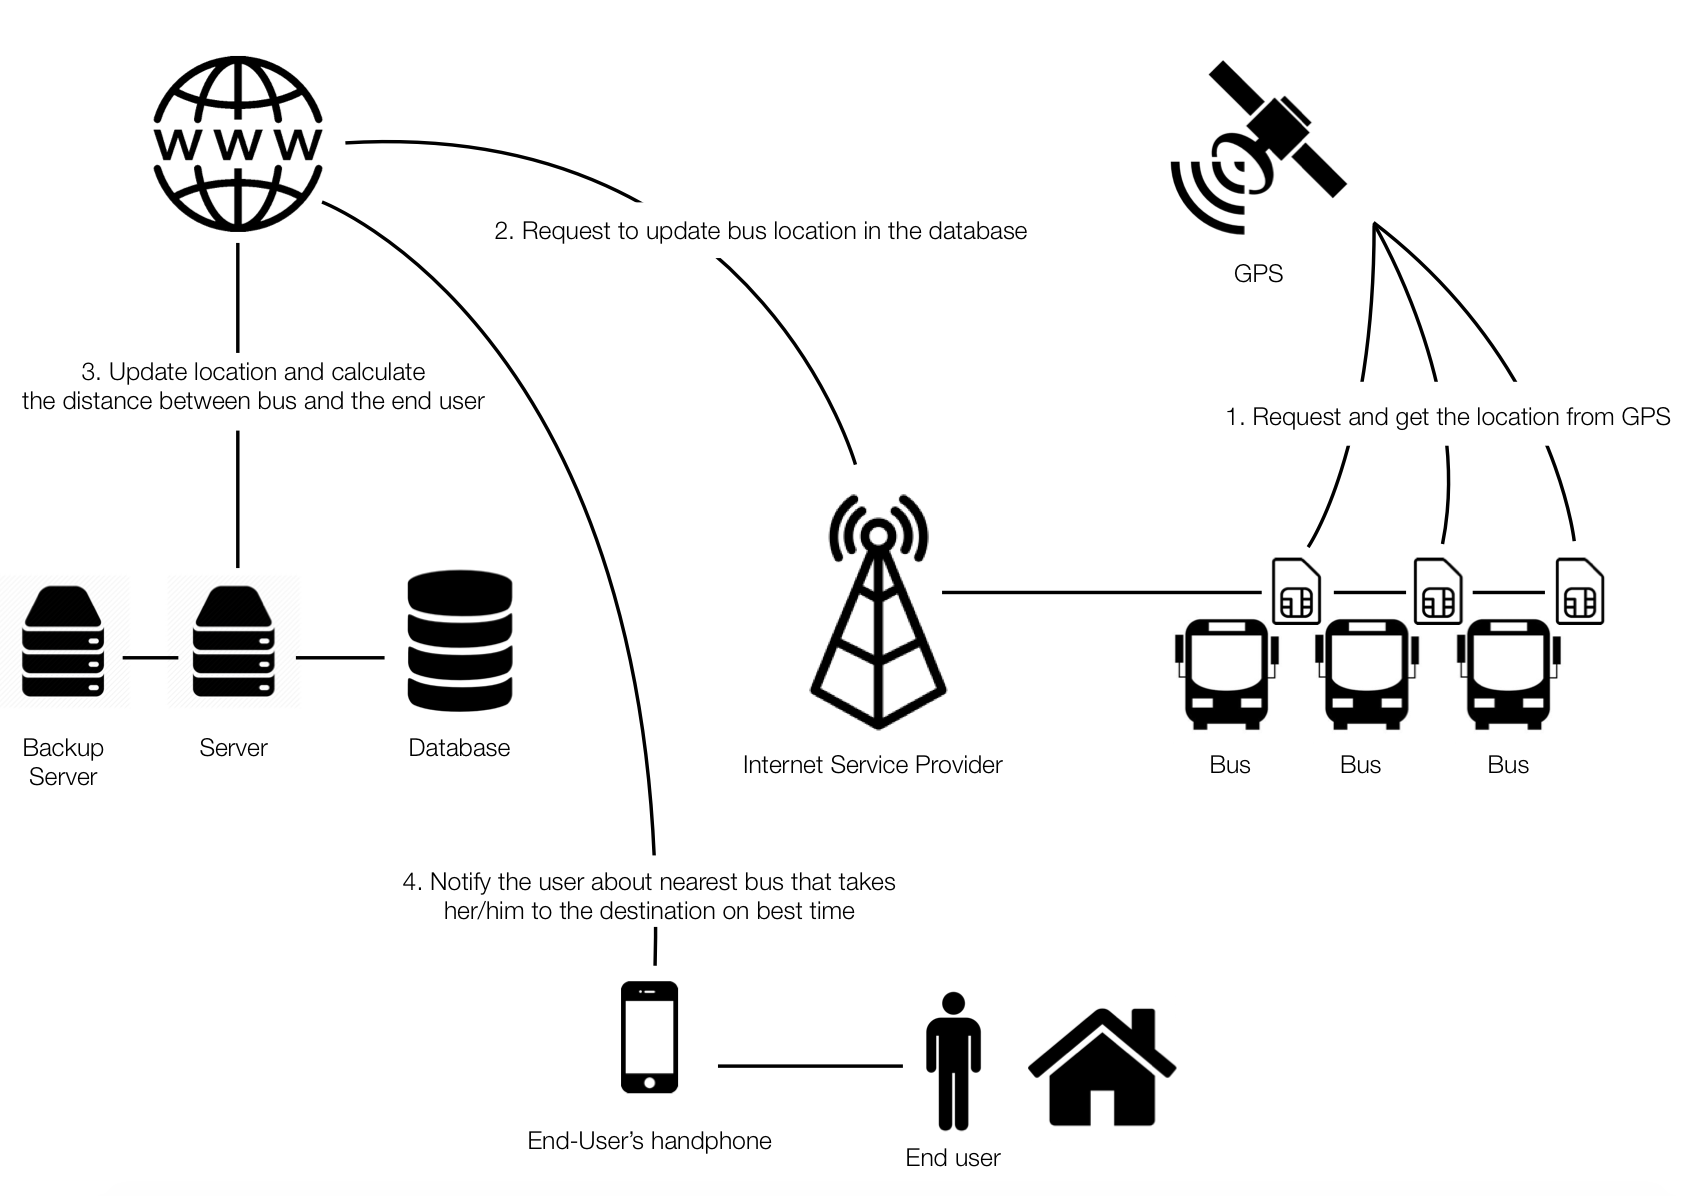
\includegraphics[scale=0.5]{Figures/FigureProposedSoftwareArchitecture.png}
	\rule{35em}{0.5pt}
	\caption[Software Architecture]{Software Architecture}
\end{figure}
\pagebreak
